% !TeX program = LaTex
% XeLaTeX or LuaLaTeX
% !TeX encoding = UTF-8 Unicode
% TEMPLATE.TEX
%
% Time-stamp: <2013-03-26 11:09 olenz>
% Update: Okt. 2020, Samuel Maier: Warnungen beseitigt, scrpage hinzugefügt, für online-PDF optimiert, konkret Verwendet.
%
% This is an extensively documented LaTeX file that shows how to
% produce a good-looking document with current LaTeX (11/2012).
%
% IMPORTANT!
%
%   Some obsolete commands and packages
% ----------|-------------------------------
% obsolete  |     Replacement in LATEX 2ε
% ----------|-------------------------------
%           | local            global/switch
% ----------|-------------------------------
% {\bf ...} | \textbf{...}     \bfseries
%     -     | \emph{...}       \em
% {\it ...} | \textit{...}     \itshape
%     -     | \textmd{...}     \mdseries
% {\rm ...} | \textrm{...}     \rmfamily
% {\sc ...} | \textsc{...}     \scshape
% {\sf ...} | \textsf{...}     \sffamily
% {\sl ...} | \textsl{...}     \slshape
% {\tt ...} | \texttt{...}     \ttfamily
%     -     | \textup{...}     \upshape
%
% DON'T USE \\ TO MAKE LINEBREAKS, INSTEAD JUST LEAVE A BLANK LINE!
%
\RequirePackage[l2tabu,orthodox]{nag} % turn on warnings because of bad style
\documentclass[a4paper,english,12pt,twoside=false]{scrartcl} %bibliography=totoc,
%
%%%%%%%%%%%%%%%%%%%%%%%%%%%%%%%%%%%%
% KOMA CLASSES
%%%%%%%%%%%%%%%%%%%%%%%%%%%%%%%%%%%%
%
% The class "scrartcl" is one of the so-called KOMA-classes, a set of
% very well done LaTeX-classes that produce a very European layout
% (e.g. titles with a sans-serif font).
% 
% The KOMA classes have extensive documentation that you can access
% via the commands:
%   texdoc scrguide # in German
%   texdoc scrguien # in English
%   
%
% The available classes are:
%
% scrartcl - for "articles", typically for up to ~20 pages, the
%            highest level sectioning command is \section
%
% scrreprt - for "reports", typically for up to ~200 pages, the
%            highest level sectioning command is \chapter
%
% scrbook  - for "books", for more than 200 pages, the highest level
%            sectioning command is \part.
%
% USEFUL OPTIONS
%
% a4paper  - Use a4 paper instead of the default american letter
%            format.
%
% german   - Use german default for packages, especially babel
%
% 11pt, 12pt, 10pt 
%          - Use a font with the given size.
%
% bibtotoc - Add the bibliography to the table of contents
%
% The KOMA-script classes have plenty of options to modify

% This allows to type UTF-8 characters like ä,ö,ü,ß
\usepackage{babel}

\usepackage[T1]{fontenc}        % Tries to use Postscript Type 1 Fonts for better rendering
\usepackage{lmodern}            % Provides the Latin Modern Font which offers more glyphs than the default Computer Modern
\usepackage[intlimits]{amsmath} % Provides all mathematical commands
\usepackage{amssymb}            % Provides amonst others the qed symbol
\usepackage{aligned-overset}    % allows for alignation of overset/underset chars by their main argument instead of the combined symbol
\usepackage{enumitem}			% allows to make listings with different enumerations, e.x. a,b,c

\usepackage{hyperref}           % Provides clickable links in the PDF-document for \ref
\usepackage{grffile}            % Allow you to include images (like graphicx). Usage: \includegraphics{path/to/file}

% Allows to set units
\usepackage[ugly]{units}        % Allows you to type units with correct spacing and font style. Usage: $\unit[100]{m}$ or $\unitfrac[100]{m}{s}$

% Additional packages
\usepackage{url}                % Lets you typeset urls. Usage: \url{http://...}
\usepackage{xspace}             % Use \xpsace in macros to automatically insert space based on context. Usage: \newcommand{\es}{ESPResSo\xspace}
\usepackage{xcolor}             % Obviously colors. Usage: \color{red} Red text
\usepackage{booktabs}           % Nice rules for tables. Usage \begin{tabular}\toprule ... \midrule ... \bottomrule

% \usepackage{fontspec}
% Source code listings
\usepackage{listings}           % Source Code Listings. Usage: \begin{lstlisting}...\end{lstlisting}
%\usepackage{lstfiracode}

\usepackage{float}

%\setmonofont[Contextuals={Alternate}]{Fira Code Regular}
%\setsansfont{Calibri}

\restylefloat{table}

\definecolor{codegreen}{rgb}{0,0.6,0}
\definecolor{codegray}{rgb}{0.5,0.5,0.5}
\definecolor{codepurple}{rgb}{0.58,0,0.82}
\definecolor{backcolour}{rgb}{0.95,0.95,0.92}

\lstdefinestyle{mystyle}{
    backgroundcolor=\color{backcolour},
    commentstyle=\color{codegreen},
    keywordstyle=\color{magenta},
    basicstyle=\ttfamily\small,
    breaklines=true
    % frame=shadowbox,
%     numberstyle=\tiny\color{codegray},
%     stringstyle=\color{codepurple},
%     basicstyle=\footnotesize,
%     breakatwhitespace=false,
%     breaklines=true,
%     captionpos=b,
%     keepspaces=true,
%     % numbers=left,
%     % numbersep=5pt,
%     showspaces=false,
%     showstringspaces=false,
%     showtabs=false,
%     tabsize=2
}

\lstset{style=mystyle}

% Add the ability to actually set the header and footer
\usepackage[footsepline=true]{scrlayer-scrpage}
\pagestyle{scrheadings}


\begin{document}

\sffamily % Use sans-serif font (I hate serif-fonts)

\newcommand{\module}{HPC\xspace}
\newcommand{\group}{Gruppe GjeSam, WS 21/22\xspace}
\newcommand{\breakln}{\mbox{} \\}

\titlehead{High Performance Computing Wintersemester 21/22, HFT Stuttgart \hfill WS 2021/2022}
\title{Abschlussprojekt}
\author{
  \textbf{\group:} \\
  Gjergji Shkurti, 357059\\
  Samuel Maier, 1002330
}
\date{\today}

\lohead{\group}
\cohead{Abschlussprojekt}
\rohead{\module, HFT Stuttgart}

\maketitle

\pagebreak

\tableofcontents

\pagebreak

\section{Motivation}

The main motivation for this project is the application of code optimization techniques learned in the high performance computing course on John Conway's "Game of Life". We started by implementing the Game of Life algorithm in a naive manner without any regards for performance. Then we used OpenMP to parallelize the algorithm. The main motivating factor here was to establish a performance baseline for future, optimized versions of the algorithm, as well as idenitify possible performance bottlenecks and ways of fixing them. By using tools such as Intel's advisor and the perf tool for Linux, we initially analyzed the different factors that could hinder the performance of the implementation such as memory bottlenecks, compute intensity and cache efficiency. Then, we looked at ways of optimizing the algorithm without the use of frameworks discussed in the course such as OpenMP and OpenCL. The idea here was to come up with creative solutions to the problem without having to rely on the funcionality of the previously mentioned frameworks and/or the use of a GPU. As discussed in the course, parallelizing bad, memory bound code can only improve the performance so much. Finally, we used the previously mentioned frameworks in two seperate parallel, optimized implementations to compare the performance to the established baseline.

\section{Game Of Life Implementation}

\subsection{Rules of the Game}

The Game of Life is a cellular automaton devised by the British mathematician John Horton Conway in 1970. The game consists of a map/board of cells which can be alive or dead. It is a zero-player game, meaning that its evolution is determined by its initial state, requiring no further input. In each successive iteration, the state of the game is determined by the state of each cell and the ammount of living/dead cells surrounding it. The generation of each state is based on the following rules:

\begin{itemize}
	\item{Any live cell with two or three live neighbours survives}
	\item{Any dead cell with three live neighbours becomes a live cell}
	\item{All other live cells die in the next generation. Similarly, all other dead cells stay dead}
\end{itemize}

\subsection{Naive Implementation}

\subsubsection{Implementation details}

We will begin with a naive and unoptimized implementation of the game to establish a performance baseline. For the naive implementation of Game of Life, the data structure depicted at listing \ref{lst:gol-naive-board-datastructure} is used to represent the board-relevant data. The board consists of a multi-dimensional vector of size \textbf{row{\_}nr x col{\_}nr}  containing integers which represent the cells themselves. Each cell can have a value of 0 (dead) or 1 (alive). Note that the datatype integer is \textbf{not} necessarily the best possible datatype to store the state of the cell, however it is chosen on purpouse to later compare the performance difference with an implementation that uses a more suited datatype.

\begin{lstlisting}[caption={Game of Life Board Datastructure},label={lst:gol-naive-board-datastructure},language=C++]
typedef struct
{
    std::vector<std::vector<int>> cell_rows;
    int row_nr;
    int col_nr;
} board_t;.
\end{lstlisting}

To test the performance of the implementation in a reproducable way, 
the initial state of the board is initialized with a glider pattern on the top left corner of the board. 
During the execution, a configurable amount of world states is generated. 
Each state can be displayed using a simplistic console based GUI. 
The displaying of the states is however deactivated and not taken into account when measuring the performance of the implementation 
as with an optimized implementation this would likely be the mayor limiting factor\\

A naive way of solving the state generation problem is to loop through each cell of the board and calculate the living neighbour count of the cell. (see listing \ref{lst:gol-naive-neighbour-counting}). Then, calculate the next cell state for each cell by taking into account the previously calculated living neighbour count and applying the rules of the game accordingly. 

\begin{lstlisting}[caption={Naive Neighbour Counting},label={lst:gol-naive-neighbour-counting},language=C++]

// Get the neighbour count of the cell at (row:col) of the board
int get_neighbour_count(int row, int col, board_t& board) {
    int neighbour_count = 0;
    int indexes[3] = { -1, 0, 1 };
    // Check col
    for (int i : indexes) {
        // Check Row
        for (int j : indexes) {
            // Avoid the current cell
            if (j || i) {
                // Add cell state (0|1) to neighbour count
                neighbour_count += cell_state_at(row + j, col + i, board);
            }
        }
    }
    return neighbour_count;
}

\end{lstlisting}

Note that it is important to make a copy of the current board state and calculate the next state for each cell by taking the copy board into account. Otherwise the current state would get corrupted during the application of the rules by the algorithm. A C++ implementation of the naive state generation algorithm can be seen in listing \ref{lst:gol-naive-generation-algorithm}. One particular consideration to keep in mind with this implementation is that for each iteration, memory for a new two dimensional vector must be allocated. We will discuss the potential performance impacts of these allocations in the following sections of this document.

\begin{lstlisting}[caption={Naive State Generation Algorithm},label={lst:gol-naive-generation-algorithm},language=C++]

int generate_cell_state(int row, int col, board_t& board){
    int cell_neighbour_count = get_neighbour_count(row, col, board);
    int cell_survives = board.cell_rows.at(row).at(col) && (cell_neighbour_count == 2 || cell_neighbour_count == 3);
    int cell_birth = !board.cell_rows.at(row).at(col) && (cell_neighbour_count == 3);
    return cell_survives || cell_birth;
}

void generate_next_board_state(board_t& current_board_state) {
    //Store current board state to avoid overriding during cell state generation
    board_t temp = current_board_state;
    // Loop through rows
    for (int row = 0; row < current_board_state.row_nr; row++) {
        // Loop through cols
        for (int col = 0; col < current_board_state.col_nr; col++) {
        	//Generate cell State
        		current_board_state.cell_rows.at(row).at(col) = generate_cell_state(row, col, temp);
        }
    }
}
\end{lstlisting}

%  TODO tables

\subsubsection{OpenMP Parallelization}

\begin{table}
\centering
\begin{tabular}{|l|l|l|l|l|l|} 
\hline
\begin{tabular}[c]{@{}l@{}}Board \\Size\end{tabular} & \begin{tabular}[c]{@{}l@{}}Serial\\Speed (ms)\end{tabular} & \begin{tabular}[c]{@{}l@{}}OpenMP\\Speed (ms)\end{tabular} & \begin{tabular}[c]{@{}l@{}}Relative\\Speedup\end{tabular} & \begin{tabular}[c]{@{}l@{}}Cache Misses\\Serial\end{tabular} & \begin{tabular}[c]{@{}l@{}}Cache Misses\\OpenMP\end{tabular} \\ 
\hline
10x10 & 206 & 188 & 1,09 & 80.053 & 105.237 \\ 
\hline
16x16 & 447 & 394 & 1,13 & 90.192 & 129.299 \\ 
\hline
32x32 & 1625 & 648 & 2,50 & 194.906 & 213.505 \\ 
\hline
64x64 & 6287 & 1921 & 3,27 & 400.519 & 421.363 \\ 
\hline
128x128 & 24501 & 7416 & 3,30 & 996.068 & 1.450.321 \\ 
\hline
256x256 & 104478 & 32401 & 3,22 & 4.546.139 & 5.557.419 \\
\hline
\end{tabular}
\caption{OpenMP Performance Comparison}
\label{tab:naive-performance-metrics}
\end{table}

The main benefit of the naive implementation of Game of Life is that computing the value of a cell in the current generation 
does not depend on the computations of the neighbouring cells. For this reason, the implementation lends itself to parallelization. 
Each thread is only responsible for reading the data of a particular board area.
All parallel threads read the current board state from the copy of the board mentioned above but none of them write in the same block of the array. 
This means that there is no need for synchronization between the threads and therefore no performance hits are incurred due to 
synchronization related overhead. 
Thus, OpenMP can be used to easily parallelize the naive state generation algorithm as seen in 
listing \ref{lst:gol-parallel-naive-generation-algorithm}. 
The only critical part is the updating of the current board state which can be done by a single thread to avoid the need for synchronization. 
Table \ref{tab:naive-performance-metrics} provides an overview of the performance difference between the serial and 
parallel implementations (8 threads) of the naive algorithm with different board sizes, on an 8 core Intel(R) Core(TM) i7-10510U CPU @ 1.80GHz processor.

\subsubsection{Limiting Factors - Cache Performance}

One limiting factor of the naive implementation is the rather poor cache performance. In Linux, cache misses can be measured by using the perf tool (sudo perf stat -e cache-misses <executable>). Table \ref{tab:naive-performance-metrics} provides an overview of the cache misses incurred when running 100000 iterations of the naive Game of Life algorithm with different board sizes and establishes a performance baseline for future comparisons. As can be seen by the results, when doubling the board size from 128x128 to 256x256, the number of cache misses for the serial implementation increases by a factor of approx. 4,5. 

\subsubsection{Limiting Factors - Memory Bottleneck}

\begin{figure}[tbh!]
	\centering
	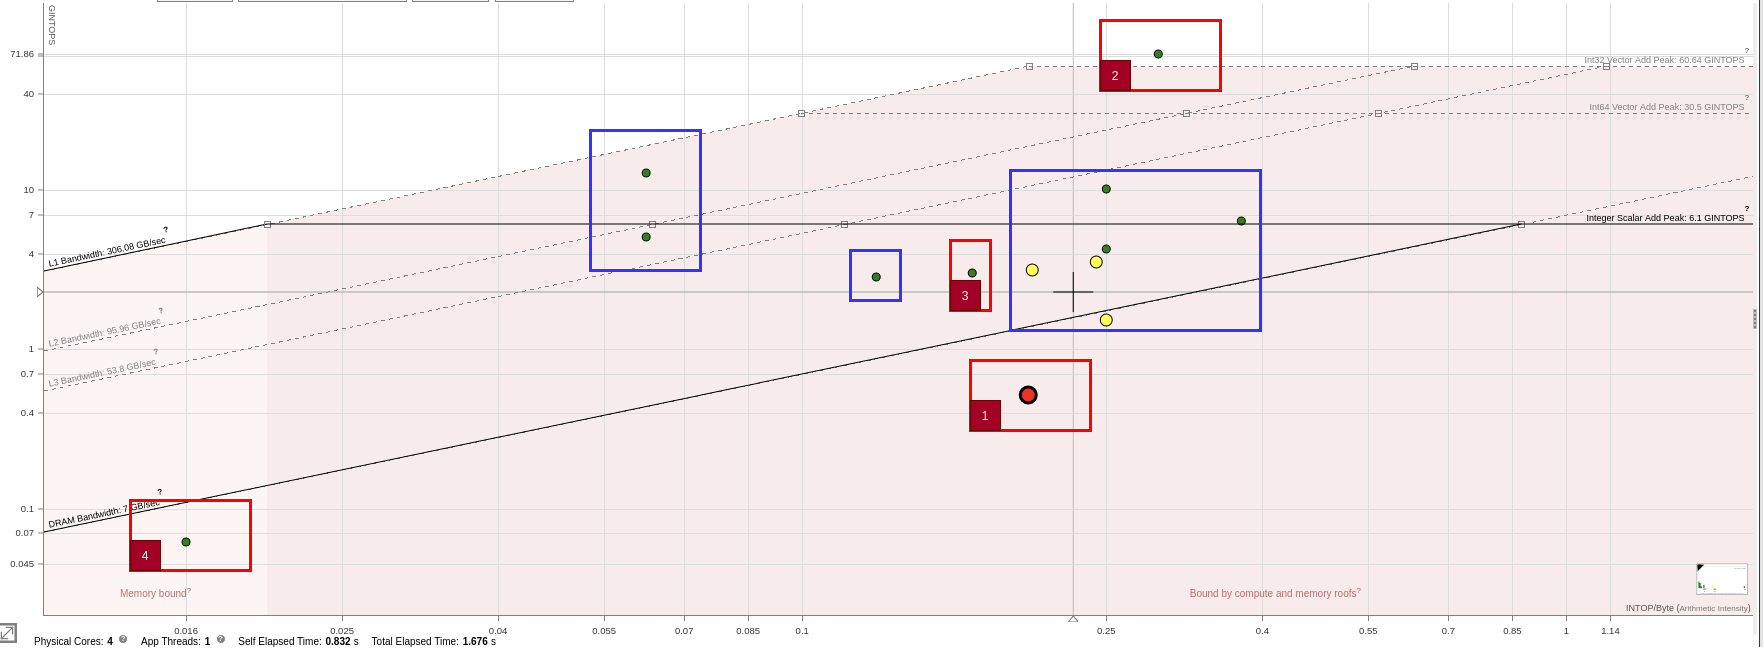
\includegraphics[width=16cm]{imgs/roofline-naive-32-100k.png}
	\caption{Roofline Analysis Results - Naive - Serial}
	\label{fig:roofline-naive-32-100k}
\end{figure}

When analyzing the performance of the naive implementation using the Roofline Model, it becomes apparent that the implementation is primarily memory bound. A lot of time is spent allocating vectors (see blue boxes in figure \ref{fig:roofline-naive-32-100k}) when making a copy of the current board state in $generate{\_}next{\_}board{\_}state{\_}(board{\_}t{\&}{\ }board)$. The compute intensity of this method as well as the method for getting the neighbour count is very low. One can also see that the largest bottleneck of the algorithm itself is the $cell{\_}state{\_}at(int{\ }row,{\ }int{\ }col,{\ }board{\_}t{\&}{\ } board)$ (1st red box in figure \ref{fig:roofline-naive-32-100k}) method which is reponsible for looking up the eight neighbouring cells of the selected cell. This particular way of looking up the neighbouring cells in the two dimensional vector is very cache inefficient as evidenced by the cache misses discussed in the previous subsection of this document. As we are memory bound and not compute bound, the benefit of parallelizing the algorithm is greatly reduced as is evidenced by the fact that the speedup factor depicted in table \ref{tab:naive-performance-metrics} plateaus after increasing the board size from 64x64 to 128x128. 

\subsection{Optimized Implementation}

As previously mentioned, the naive algorithm lends itself well to parallelization with a framework such as OpenMP. However, the algorithm itself has a low compute intensity and is rather inefficient in regards to memory and cache performance. As such, the performance gains from parallelizing the algorithm by using OpenMP are very restricted. In this chapter, an optimized version of the algorithm and a better way of representing the cell-relevant data to increase cache performance are discussed. The implementation aims to solve the Game of Life state generation problem more efficiently than the previous one, without the use of parallelization.

\subsubsection{Optimized Data Representation}

\begin{figure}[tbh!]
	\centering
	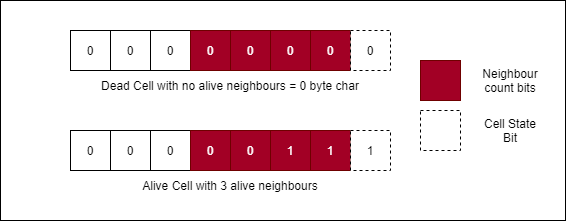
\includegraphics[width=16cm]{imgs/cell-state.png}
	\caption{Cell State Char}
	\label{fig:cell-state}
\end{figure}

Another approach to solving the state generation problem is to encode both the cell state and the number of living neighbours a cell has into a single datatype. Then, when manipulating the state of a cell, one can accordingly increment or decrement the number of living neighbours for each of the surrounding cells. Lets consider cell-relevant data. A cell has a state (dead/alive) which can be encoded into a single bit (1/0). It can have a minimum of 0 living neighbours and a maximum of 8, which can be represented by using only 4 bits. So, to store all relevant cell data, we need a total of 5 bits. We can store all cell-relevant data in the first 5 bits of an unsigned char (see figure \ref{fig:cell-state}), and ignore the remaining 3 bits. Keeping this in mind, we can store the state of all cells of the board into a one dimensional array of unsigned chars. In doing so, we avoid the performance hits incurred due to the vector allocations in the first implementation.

By using a smaller datatype, we greatly reduce the ammount of memory needed to store our board states compared to the previous naive implementation, where an integer was used to store only the cell state. The other benefits of representing our data in this way are discussed in the following subsection of this document. Listing \ref{lst:gol-optimized-datastructure} depicts the optimized structure of storing all board-relevant data.

\begin{lstlisting}[caption={Parallel Naive State Generation Algorithm},label={lst:gol-optimized-datastructure},language=C++]

typedef struct
{
    u_char* cells = nullptr;
    u_int rows;
    u_int cols;
    u_int length;
} board_t;

\end{lstlisting}

\subsubsection{Optimized Board State Generation Algorithm}

\begin{figure}[tbh!]
	\centering
	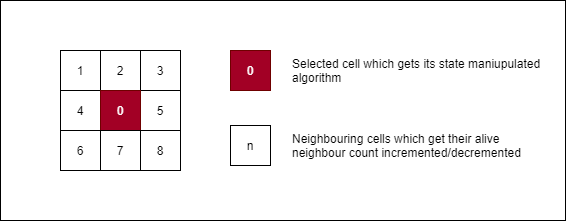
\includegraphics[width=16cm]{imgs/cell-algo.png}
	\caption{Optimized Generation Algorithm}
	\label{fig:cell-algo}
\end{figure}

As shown in figure \ref{fig:cell-state}, a dead cell with no alive neighbours is simply a 0 byte. These cells can never change their state. We can skip applying the rules of the game to all cells that fulfill the requirement of being 0 bytes. This has two benefits: Firstly, our algorithm gains a significant performance increase as it can simply access the cell via a pointer and check whether its dereferenced value is 0. If that is the case, it can skip analyzing the cell and move on to its neighbour. In doing so, we improve cache performance as the amount of times we need to lookup the surrounding cells in our array is greatly decreased. Secondly, over time, the game of life gravitates towards a sparse state. This means, on a randomly initialized board, the further we are in our iterations, the larger the number of dead cells without any living neighbours is. Because our algorithm simply skips such cells, its performance gain becomes larger the further we are in our iterations.

Listing \ref{lst:gol-optimized-manipulation} depicts the method for setting the cell of a state to dead and deincrementing the neighbour counts of its surrounding neighbours. Bitwise manipulation is used to set the intial bit of the unsigned char representing the cell data to 0. Then, bitwise manipulation is used to reduce the alive neighbour count of each surrounding cell by one. Setting the cell state to alive is similar. The only difference is that the first bit is set to 1 ($*(cell_ptr) |= 0x01$)  and the count of each neighbour is incremented by one ($*(cell_ptr + y + x) += 0x02$).

\begin{lstlisting}[caption={Parallel Naive State Generation Algorithm},label={lst:gol-optimized-manipulation},language=C++]
void kill_cell(board_t& board, const u_int& row, const u_int& col) {
    // index 1d array as 2d array
    u_char* cell_ptr = board.cells + (col * board.cols) + row;
     // kill the cell by setting first bit to 0
    *(cell_ptr) &= ~0x01;
    // Handle indexes if the cell is on the edges of the board
    int x_left, x_right, y_above, y_below;
    get_wrap_indexes(board, row, col, x_left, x_right, y_above, y_below);
    // Deincrement the neighbour count of all surrounding cells since the cell died
    *(cell_ptr + y_above + x_left) -= 0x02;
    *(cell_ptr + y_above) -= 0x02;
    *(cell_ptr + y_above + x_right) -= 0x02;
    *(cell_ptr + x_left) -= 0x02;
    *(cell_ptr + x_right) -= 0x02;
    *(cell_ptr + y_below + x_left) -= 0x02;
    *(cell_ptr + y_below) -= 0x02;
    *(cell_ptr + y_below + x_right) -= 0x02;
}
\end{lstlisting}

Listing \ref{lst:gol-optimized-algo} depicts the optimized state generation algorithm. As previously discussed, we initially check if the selected cell is a 0 byte and if that is the case, we skip the application of the rules. If the requirement for skipping is not fulfilled, the alive neighbour count of the cell is acquired by using a bitwise shift operation on the unsigned char representing the cell-relevant data. If the data of the unsigned char is shifted by one to the right, the state bit becomes a carry bit. Therefore, the only remaining data in the unsigned char are the 4 bits representing the alive neighbour count of the selected cell. Depending on this number, we apply the rules of the game to the cell and update all neighbouring cells accordingly.

\pagebreak

\begin{lstlisting}[caption={Parallel Naive State Generation Algorithm},label={lst:gol-optimized-algo},language=C++]
void generate_next_board_state(board_t& board, board_t& temp_board) {
    memcpy(temp_board.cells, board.cells, board.length);
    for (u_int index = 0; index < board.rows * board.cols; index++) {
        auto lookup_cell_ptr = temp_board.cells + index;
        if (*lookup_cell_ptr == 0)
            continue;
        auto nb_count = (*lookup_cell_ptr) >> 1;
        bool is_alive = (*lookup_cell_ptr) & 0b01;
        if (is_alive) {
            // if the cell stays alive, skip
            if (2 <= nb_count && nb_count <= 3)
                continue;
            u_int col = index % board.rows;
            u_int row = index / board.rows;
            // // kill the cell
            kill_cell(board, col, row);
        } else {
            // cell only gains life when it has precisely 3 neighbours
            if (nb_count != 3)
                continue;
            u_int col = index % board.rows;
            u_int row = index / board.rows;
            spawn_cell(board, col, row);
        }
    }
}
\end{lstlisting}

Note that the cache performance of this implementation, tested on a board containing a single glider, is much better than the previous naive implementation. (see table \ref{tab:optimized-cache-misses}). When analyzed with Intel's Advisor, this implementation was significantly less memory bound than the previous one and had a higher compute intensity. Despite the fact that the implementation is not parallelized, because of the increased memory and cache efficiency ,the optimized state generation algorithm performs much better than the naive implementation, particularly on smaller board sizes. That being said, in contrast to the naive implementation, computing the value of each state is now dependent on the computations of the neighbouring cells. This means that parallelizing the optimized implementation requires a significant amount of synchronization overhead, which is of course a large performance bottleneck. 

\begin{table}
\centering
\begin{tabular}{|l|l|l|l|} 
\hline
\begin{tabular}[c]{@{}l@{}}Board \\Width\end{tabular} & \begin{tabular}[c]{@{}l@{}}Speed~\\(ms)\end{tabular} & \begin{tabular}[c]{@{}l@{}}Cache\\Misses\end{tabular} & \begin{tabular}[c]{@{}l@{}}Speedup relative \\to the OpenMP \\Naive Implementation\end{tabular} \\ 
\hline
10x10 & 10 & 57.109 & 18,8 \\ 
\hline
16x16 & 21 & 76.464 & 18,76 \\ 
\hline
32x32 & 68 & 89.584 & 9,52 \\ 
\hline
64x64 & 253 & 84.346 & 7,59 \\ 
\hline
128x128 & 1044 & 108.983 & 7,10 \\ 
\hline
256x256 & 4273 & 206.050 & 7.58 \\
\hline
\end{tabular}
\caption{Performance - Optimized}
\label{tab:optimized-cache-misses}
\end{table}

\pagebreak

\subsection{OpenCL Implementation}

To use OpenCL at all we had to do quite a bit of work, since we had a Makefile based build process,
so we had build the Application using mostly \verb|wsl|, but passing a GPU to \verb|wsl| is no small feat. 
So we installed a native Linux OS.

We were also triggered to rethink the implementation fundamentally for OpenCL, 
since it has explicit memory tiers compared to the CPU with implicit caching.

OpenCL prefers to group parts of the algorithm in 2 levels, one individual problem - \verb|Work-Item|s - 
and a group of them together - \verb|Work-Group|. Items in a group can coordinate with shared memory, 
and access to that memory is usually a magnitude faster than access to global memory, 
that is shared by all Groups (so shared among the entire algorithm).\\
We want to utilize this of course. But another problem is the execution and branching. 
All work-items in a work-group must be assumed to be executed together with one instruction pointer.\\
This means that for starters the slowest work-item will determine the combined execution speed. 
But the coupling is stronger than that. If the code includes branching, AND both branches get executed,
these branches must be executed AFTER one another, because of the single instuction pointer per work-group 
(in reality these assumtions are not always true, but work-items and groups are meant to be abstractions on 
vendor-specific architectures, that usually behave similar).

\subsubsection{Memory locality and branching}

Since every cell, upon its calculation, needs to look up its neibours and its own value, in one generation the value of 
a cell needs to be looked up 9 times, 8 times by the neighbours, once by itself. So we want to cache this.
We also want to keep down the number of lookups in global memory per work-item, as that is assumed to be a magnitude slower 
than local memory - so the memory shared among a work-group.\\
Especially because of the shared instruction pointer we want to reduce the number of memory lookups.
The best case would be one memory lookup per item, on the same code-line.\\
To do that in a work-group that is smaller than the board, we need more work-items than Game of Life (GoL) Cells written to in that group.
The first idea we had was to add another dimension to the work-group, where the 3rd dimension is meant to do the additional loading. 
But that is hard to organize both by us, and by the GPU, leading to additional load and massive slow-down because of the single instruction pointer.
We can also only execute a single kernel in one work-group, because of the single instruction pointer.

\begin{center}
    \captionof{figure}{Memory-access pattern with work-groups}
    \label{fig:cl-mem-access}
    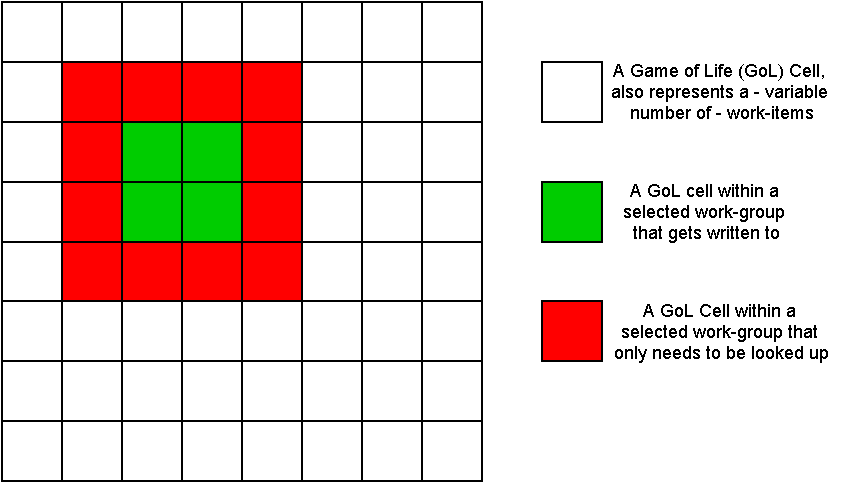
\includegraphics[width=\linewidth]{imgs/opencl_mem_access.drawio.pdf}
\end{center}

The simple solution we eventually recognized is to have additional work-items around the border of the area that is worked on by the work-group.
The sole purpose of these work-items is to load the value of their respective GoL cell into the local memory. 
But because they do that exactly the same way as the other work-items, they dont slow down them, and total execution of the work-group is faster.
\autoref{fig:cl-mem-access} is demonstrating this on a simple board. 
In that example the board is sized $8^2$, the block-size that a work-group works on is $2^2$, but the work-group has the size $(2 + 2\times 1)^2 = 4^2$.

\autoref{lst:opencl-kernel-source} shows the source-code for this OpenCL implementation.

We also implemented another version (V2), that uses 2 seperate memory buffers, and gets rid of the global memory barrier in the kernel

\subsubsection{Platform}

These findings were recorded on a Tower PC with the Linux-Kernel 5.15, Nvidia Driver 495.44, a Nvidia GTX 1070 and an AMD Ryzen R5 3600 (both well cooled), using the Nvidia provided OpenCL 3.0 implementation.

For further experiments we also installed the Portable Computing Language (PoCL), which is an OpenCL implementation that compiles via LLVM to run on the CPU.

We also ported the OpenCL implementation V2 of our Programm as accurately as possible to OpenMP (porting V1 wasn't possible).

\subsubsection{Performance Results}

A performance comparison of the OpenCL implementation with the other implementations can be found in \autoref{chap:summary}. \\
First of all we experimented with the \verb|BLOCK_SIZE|.
This number determines how many workitems are in a workgroup - there are $(\verb|BLOCK_SIZE| + 2)^2$ workitems in a workgroup.

We noticed that scaling our \verb|BLOCK_SIZE| beyond 12 lead to the error \verb|CL_OUT_OF_RESOURCES|,
meaning this would allocate too much memory per work-group on the device, so this was a hard upper limit.

We choose these high board-sized because otherwise we'd get too fast times, that were unsafe to compare.
We choose these specific values because they all are divided by the \verb|BLOCK_SIZE|s we choose.

\begin{table}[]
\centering
\begin{tabular}{l||l|l|l|l|l|l|l}
    \verb|BLOCK_SIZE|    & 12   & 10   & 8    & 6    & 5    & 4    & 2    \\ \hline \hline
    execution time v1 /s & 13.6 & 12.0 & 9.60 & 8.77 & 10.6 & 15.8 & 36.4 \\ \hline
    execution time v2 /s & 9.34 & 9.60 & 8.10 & 7.86 & 9.86 & 15.4 & 37.5 \\
\end{tabular}
\caption{The execution time of both OpenCL versions as they scale with block-size, at a board-size of $960^2$, and 100k generations}
\label{tab:blocksize-scaling1}
\end{table}

\begin{table}[]
\centering
\begin{tabular}{l||l|l|l|l}
    \verb|BLOCK_SIZE|    & 12   & 8    & 6    & 5    \\ \hline \hline
    execution time v1 /s & 10.5 & 9.42 & 8.01 & 9.74 \\ \hline
    execution time v2 /s & 7.30 & 6.65 & 6.26 & 7.83 \\
\end{tabular}
\caption{The execution time of both OpenCL versions as they scale with block-size, at a board-size of $240^2$, and 1000k generations}
\label{tab:blocksize-scaling2}
\end{table}

As one can see in these charts, the ideal \verb|BLOCK_SIZE| was at 6, meaning there were 36 work-items per work-group.
We suspect that this is because of our GPU can execute 32 threads ("warps" in Nvidia Terminology).
Beyond that we saw a slight decrease in speed, until the device was unable to run because of the error mentioned above.
We were slightly surprised that there were no issues with thread contention or similar, but these threads were probably just distributed on seperate "Multiprocessor"s, with the performance decrease coming from the shared memory.
Below this we saw relatively fast slow-downs, as this meant that our algorithm had a massive increase in the relative amount of work-items that are only there to load memory.

We also saw, as expected, a speedup from the V1 of the kernel, with a global memory barrier, to V2 without one but 2 buffers. Surprisingly that difference was fairly small, and doesn't seem to scale overly differently with eg- problemsize.

\section{Summary, conclusions and potential avenues}
\subsection{Summary}
\label{chap:summary}

\begin{table}
    \centering
    \begin{tabular}{|l|l|l|l|l|l|l|l|}
    \hline
    \begin{tabular}[c]{@{}l@{}}Board\\Size\end{tabular} & \begin{tabular}[c]{@{}l@{}}OpenCL\\v1\end{tabular} & \begin{tabular}[c]{@{}l@{}}OpenCL\\v2\end{tabular} & \begin{tabular}[c]{@{}l@{}}OpenCL\\v2 PoCL\end{tabular} & \begin{tabular}[c]{@{}l@{}}Optimized\\Char Cellmap\end{tabular} & \begin{tabular}[c]{@{}l@{}}OpenMP\\Naive\end{tabular} & \begin{tabular}[c]{@{}l@{}}OpenMP\\OpenCL\\v2 Port\end{tabular} \\
    \hline
    120 & 373 & 264 & 6939 & 739 & 116958 & 1895 \\
    \hline
    480 & 2997 & 2096 & 36447 & 11690 & N/A & 25105 \\
    \hline
    \end{tabular}
    \caption{General Performance Comparison}
    \label{tab:general-performance-comparison}
\end{table}
    
In total the variants we developed on our GPU were the fastest with quite a distance to the rest.

But GPUs are designed for loads like that, and creating that programm was still quite a difficult feat.

Considering that it runs only on a single core, the optimized \verb|char-cell| variant is impressively fast in comparison to the others, and in terms of computational and probably also energy efficiency is hard to beat.

It still beats our best OpenMP variant. That was the port of our OpenCL V2 implementation to OpenMP, handily beating out our first naive OpenMP variant.

The likely reason is that the OpenCL implementations have better cache locality and, while less efficient in computation, spread out the work more.

The reordering of the board into the block gets worked on by all CPU cores, and after that most cores work on their cell.

The execution of our OpenCL implementations on our CPU, using the Portable Computing Language, were interestingly far slower than our OpenMP port.
We are uncertain whether this is due to PoCL being a potentially inefficient implementation, or due to general OpenCL overhead, or something else entirely.

\subsection{Potential avenues}

We had some difficulties and eventually gave up on porting our char-optimized version of the game to OpenCL or OpenMP. 
The reason is the reconciliation of the neighbor-counts at the borders.
But perhaps we just didnt find the right solution, so that would be worth looking into.
On OpenCL however it has to be noted that the speedup due to less computation will not be present due to the single stack pointer. 
But it probably still reduces memory access.

Our fastest OpenMP implementation was the OpenCL port.
Because it aims to be as straight a port of the OpenCL variant as possible to be compareable, 
it has a number of additional optimizations that would be possible, that we sadly didnt get to.

Our OpenCL implementations worked fairly well, but we didnt get to really delve into the profiling that is possible there, 
using it we might find some optimizations that quite possibly massively increase performance.

We did not dive into the intricacies of the tools used to measure the performance of our implementations such as
Intel's Advisor and the perf tool. Intel's Advisor in particular was a rather feature rich software offering, amongst other things,
optimization recommendations such as loop vectorization and pragma directives that could help the compiler further
optimize the code. Most of these features were only compatible with an intel compiler however, so we decided to not focus on them.
We had issues using Intel Advisors Memory Access Pattern Analysis feature and could not use it
to measure the cache performance of each individual loop/function of our implementations. We decided to use perf tool for this reason
but limited ourselves to the basic features such as measuring cache misses. Future work could include a deeper cache performance analysis
as well as a better roofline model performance analysis of \textbf{each implementation} using Intel's Advisor. It would also be worth looking
into loop vectorization to optimize the performance of our implementations. \breakln

One feature that we considered implementing, but didn't get to, was the recognition of loops, or some other detection of "its the same from now on".

One optimization idea we had considering that feature, was the use of a hashing algorithm to store current board states.
The idea here was to use the hashed board states to identify when the game of life state was identical to that of a previous generation.
In these cases, the board state for the next generation could be reconstructed from the hashed value instead of by applying the algorithms discussed
in this document.

\subsection{Footnotes}

One issue that we noticed close to the end, is that nearly all of our benchmarks were made using a board with just one glider.

The OpenCL variants are probably not strongly effected by this,
but due to its "output sensitive" computation requirement the \verb|char-cell| optimized variant is influenced by this.

\section{Source Code}
Apart from the listings we included for source code, the remaining ~4k lines of this Project can be found at \href{https://github.com/GjergjiSh/hpc-game-of-life}{Github (https://github.com/GjergjiSh/hpc-game-of-life)}. 

\section{Appendix}
\begin{center}
    \captionof{figure}{Sourcecode of the kernel for our OpenCL implementation}
    \label{lst:opencl-kernel-source}
    \lstinputlisting[language=C++]{../src/opencl/gol_work_group.cl}
\end{center}


\begin{lstlisting}[caption={Parallel Naive State Generation Algorithm},label={lst:gol-parallel-naive-generation-algorithm},language=C++]
void game_of_life_loop_omp(board_t& board, board_t& temp, int generations, int display) {
#pragma omp parallel num_threads(8)
    {
        num_threads = omp_get_num_threads();
        for (int gen = 0; gen < generations; gen++) {
#pragma omp for
            for (int row = 0; row < board.row_nr; row++) {
                for (int col = 0; col < board.col_nr; col++) {
                    int alive_neighbours = get_neighbour_count(row, col, board);
                    int cell_survives = board.cell_rows.at(row).at(col) && (alive_neighbours == 2 || alive_neighbours == 3);
                    int cell_birth = !board.cell_rows.at(row).at(col) && (alive_neighbours == 3);
                    temp.cell_rows.at(row).at(col) = cell_survives || cell_birth;
                }
            }
#pragma omp master
            {
                board.cell_rows.swap(temp.cell_rows);

                if (display) {
                    display_board_state(board);
                }
            }
#pragma omp barrier
        }
    }
}
\end{lstlisting}

\end{document}